\documentclass{article}
% if you need to pass options to natbib, use, e.g.:
% \PassOptionsToPackage{numbers, compress}{natbib}
% before loading nips_2016
%
% to avoid loading the natbib package, add option nonatbib:
% \usepackage[nonatbib]{nips_2016}

%\usepackage{nips_2016}

% to compile a camera-ready version, add the [final] option, e.g.:
\usepackage[final,nonatbib]{nips_2016}

%\usepackage[utf8]{inputenc} % allow utf-8 input
\usepackage[T1]{fontenc}    % use 8-bit T1 fonts
\usepackage{hyperref}       % hyperlinks
\usepackage{url}            % simple URL typesetting
\usepackage{booktabs}       % professional-quality tables
\usepackage{amsfonts}       % blackboard math symbols
\usepackage{nicefrac}       % compact symbols for 1/2, etc.
\usepackage{microtype}      % microtypography
\usepackage[shortlabels]{enumitem}
\usepackage{color}
\usepackage{ragged2e}
\usepackage[square,sort,comma,numbers]{natbib}
\usepackage{amsmath,amsthm,amssymb,amsfonts}
\newtheorem{theorem}{Theorem}
\newtheorem{proposition}{Proposition}
\newtheorem{corollary}{Corollary}

\newcommand{\EE}{\mathbb{E}}
\newcommand{\PP}{\mathbb{P}}
\newcommand{\Ss}{\mathcal{S}}
\newcommand{\Ii}{\mathcal{I}}
\newcommand{\Ee}{\mathcal{E}}
\newcommand{\Rr}{\mathcal{R}}
\DeclareMathOperator*{\argmin}{arg\,min}
\DeclareMathOperator*{\argmax}{arg\,max}

%\title{Bayes-Optimal Intrinsically Motivated Learning v.s. Empowerment Maximisation}
%\title{Deriving Intrinsic Motivation from \\ Uncertainty about Future Goals}
\title{A Bayesian Approach to Intrinsically\\Motivated Reinforcement Learning}

\author{
 Jeffrey Negrea\\
 Department of Statistical Sciences\\
 University of Toronto\\
 \texttt{negrea@utstat.toronto.edu}
 \And
 David Duvenaud\\
 Department of Computer Science\\
 University of Toronto\\
 \texttt{duvenaud@cs.toronto.edu}
}


\usepackage{tikz}
\usetikzlibrary{arrows,shapes,trees}

\tikzstyle{title} = [rectangle, rounded corners, minimum width=2cm, minimum height=1cm, text centered, draw=black]

\tikzstyle{start} = [rectangle, rounded corners, minimum width=2cm, minimum height=1cm, text width=2cm, text centered, draw=black, fill=red!30]

\tikzstyle{stop} = [rectangle, rounded corners, minimum width=2cm, minimum height=1cm, text centered, draw=black, fill=green!30]


\tikzstyle{io} = [trapezium, trapezium left angle=80, trapezium right angle=100, minimum width=2cm, minimum height=1cm, text centered, draw=black, text width=2cm, fill=blue!30]

\tikzstyle{process} = [rectangle, minimum width=2cm, minimum height=1cm, text centered, text width=2cm, draw=black, fill=orange!30]

\tikzstyle{prior} = [rectangle, minimum width=2cm, minimum height=1cm, text centered, text width=2.1cm, draw=black, fill=purple!30]

\tikzstyle{decision} = [diamond, minimum width=1cm, minimum height=1cm, text centered, draw=black, fill=purple!30]

\tikzstyle{arrow} = [thick,->,>=stealth]

\begin{document}
\maketitle

\begin{abstract}
Intrinsically motivated reinforcement learning asks how agents act when motivated by an internal reward system, and how such a reward system should be structured. 
We suggest a simple approach that considers that intrinsic motivation arises from uncertainty about the future goals of an agent.
We formalise this approach using Bayesian decision theory, and show that it meets desired characteristics for intrinsic motivation. 
We also compare our approach to the recently-proposed empowerment metric, and give a simple example where empowerment fails to choose the optimal policy.
\end{abstract}

\section{Introduction and Related Work}
%Reinforcement Learning is the process by which an agent learns about an environment through interaction with the environment in order to discover how to achieve a prescribed goal.
%Often the agent is conceptualised to interact with the environment across a discrete time horizon.
%Two common formulations considered are a sequence of \textit{episodes} each executed over a finite time horizon, and a single episode executed over a possibly infinite time horizon. 
%The agent's goal is usually assumed to be to maximise its expected reward or expected discounted reward.
%The optimal strategy in such a formulation then may be determined by the Bellman optimality equations \cite{sutton1998reinforcement}.
%Reinforcement learning has been successfully applied to a variety of problems in robotics \cite{mcallister2016data,finn2016deep,christiano2016transfer}, video game A.I. \cite{mnih2015human}, and medical decision making \cite{krishnan2016structured}.
A key component of traditional reinforcement learning frameworks is that the mechanism by which the actor receives rewards is fixed and is pre-prescribed as part of the environment.
% though it may not be known \textit{a priori} by the actor.
Intrinsically motivated reinforcement learning aims to generalise the notion of reward functions for reinforcement learning problems by shifting the reward system from being part of the environment to being partially or completely part of the actor, and/or by not requiring the reward system to be fixed or pre-prescribed. This is often interpreted as allowing the actor to be motivated not only by achieving standardised goals, but also for having improved its model of the environment, and is often compared to the way in which humans and animals learn through playing and experimentation \citep{oudeyer2008can,schmidhuber2010formal}. 
%is specified in advance (though still not known to the actor). 

However, there is a divergence in the literature as to what it means to be intrinsically motivated; while it is generally established that the core component of intrinsic motivation is that the reward system used to establish the optimal policy is internal to the actor, there exist multiple distinct interpretations of how reward systems are related to the environment. The first interpretation asserts that there is a fixed underlying external fitness function (e.g. reproductive success) on the space of actor trajectories. This is described in Singh \textit{et al.} \cite{singh2010intrinsically}, where the authors propose that the reward system used to drive the agent's behaviour should be internal to the agent and the focus of their approach is the search for the internal reward function which yields the highest expected fitness. This may be interpreted as a way of smoothing the external reward system (fitness) in order to avoid overly greedy, short-sighted strategies. This may be viewed as an abstraction or generalisation of the Q-learning discounted future reward framework.
 
\begin{figure}[h]
\centering
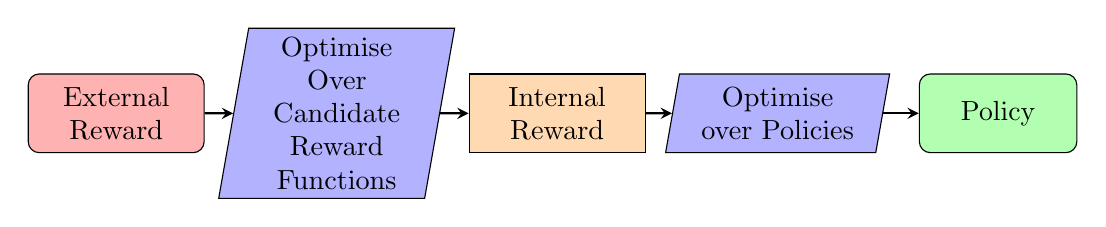
\begin{tikzpicture}[node distance=1cm]
\node (extR) [start] {External Reward};
\node (optE) [io, right of=extR,xshift=1.8cm] {Optimise Over Candidate Reward Functions};
\node (intR) [process, right of=optE,xshift=1.8cm] {Internal Reward};
\node (optT) [io, right of=intR,xshift=1.8cm] {Optimise over Policies};
\node (pol)  [stop, right of=optT,xshift=1.8cm] {Policy};

\draw [arrow] (extR) -> (optE);
\draw [arrow] (optE) -> (intR);
\draw [arrow] (intR) -> (optT);
\draw [arrow] (optT) -> (pol);
\end{tikzpicture}
\caption{Intrinsic Motivation as per Singh \textit{et al.}} \label{fig:M1}
\end{figure}

The second interpretation, as per Schmidhuber \cite{schmidhuber2010formal}, posits that reward systems are split (possibly non-linearly) into internal and external components, and that the internal component of motivation is derived from quality of the learned environmental model. The heuristic qualities of the internal reward component in this framework are listed in section 2. Model quality in this framework is, in some instances, identified with the model's efficiency as a compressor of the data history. Incremental internal reward from time $t$ to time $t+1$ is measured based on (a possibly non-linear) notion of the improvement in model quality between the model fit on the first $t$ observations and the model fit on all $t+1$ observations, when performance is assessed with respect to all $t+1$ observations.

\begin{figure}[h]
\centering
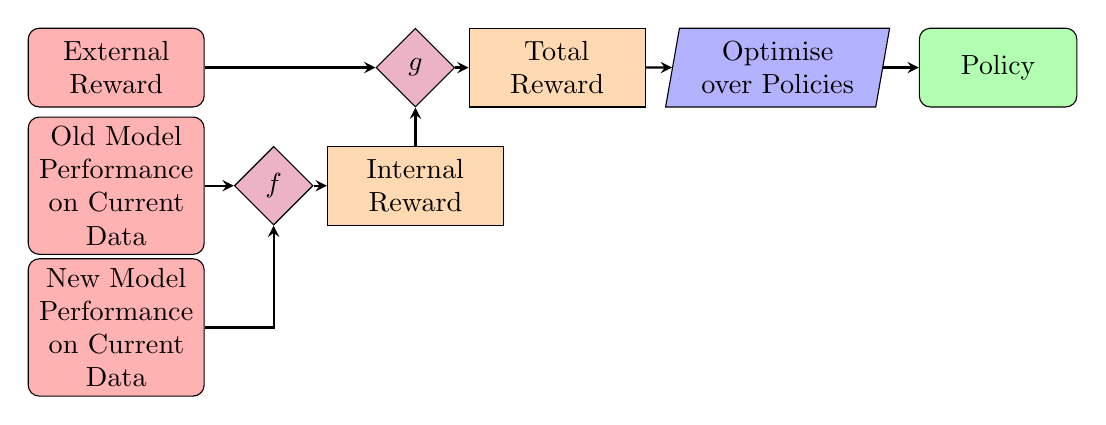
\begin{tikzpicture}[node distance=1cm]
\node (extR) [start] {External Reward};
\node (oldM) [start, below of=extR,yshift=-.5cm] {Old Model Performance on Current Data};
\node (newM) [start, below of=oldM,yshift=-.8cm] {New Model Performance on Current Data};
\node (f) [decision, right of=oldM,xshift=1cm] {$f$};
\node (intR) [process, right of=f,xshift=.8cm] {Internal Reward};
\node (g) [decision,above of=intR,yshift=.5cm] {$g$};
\node (totR) [process, right of=g,xshift=.8cm]{Total Reward};
\node (optT) [io, right of=totR,xshift=1.8cm] {Optimise over Policies};
\node (pol)  [stop, right of=optT,xshift=1.8cm] {Policy};

\draw [arrow] (extR) -> (g);
\draw [arrow] (oldM) -> (f);
\draw [arrow] (newM) -| (f);
\draw [arrow] (f) -> (intR);
\draw [arrow] (intR) -> (g);
\draw [arrow] (g) -> (totR);
\draw [arrow] (totR) -> (optT);
\draw [arrow] (optT) -> (pol);
\end{tikzpicture}
\caption{Intrinsic Motivation as per Schmidhuber} \label{fig:M2}
\end{figure}

The third interpretation, \cite{mohamed2015variational,salge2014empowerment}, establishes that reward systems exist external to the actor, however they are unknown and stochastic. Internal motivation is then formulated as a utility system that is optimised in order to prepare for an unknown future goal/reward system. It is this notion of intrinsic motivation that we will focus on for this project. 

The recently-introduced measure of \emph{empowerment}~\citep{mohamed2015variational, salge2014empowerment} approaches the problem using information-theoretic metrics, aiming to maximise notions of dependence between the actions taken and the resultant state. Specifically, empowerment-based intrinsic motivation, as discussed in \citep{mohamed2015variational}, optimises the mutual information of the action distribution and the resulting outcome.
Heuristically, as described in \cite{salge2014empowerment}, empowerment measures the amount by which an actor can influence the outcome of a game.
It is $0$ when the all of the viable actions have identical influence on the resulting state, and is positive otherwise. However, as shown in figure 3, there is no connection between the empowerment-based internal reward system or its resulting policy and the external reward system. This is unsatisfactory as agents will not be driven to achieve real goals through any amount of learning. The expected reward framework we introduce in section 3 addresses the same class of problems as empowerment, but has an architecture which accounts for the external reward system, as shown in figure 4. 

\begin{figure}[h]
\centering
\begin{tikzpicture}[node distance=1cm]
\node (extR) [start] {External Reward (Unknown \& Random)};
\node (intR) [process, right of=optE,xshift=1.8cm] {Internal Reward};
\node (optT) [io, right of=intR,xshift=1.8cm] {Optimise over Policies};
\node (pol)  [stop, right of=optT,xshift=1.8cm] {Policy};

\draw [arrow] (intR) -> (optT);
\draw [arrow] (optT) -> (pol);
\end{tikzpicture}
\caption{Intrinsic Motivation as per Empowerment Maximisation} \label{fig:M3}
\end{figure}

\begin{figure}[h]
\centering
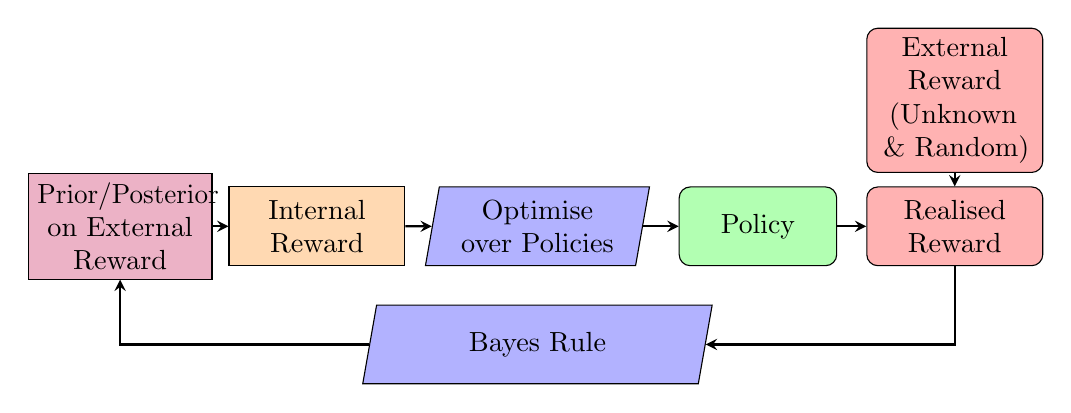
\begin{tikzpicture}[node distance=1cm]
\node (pi)   [prior] {Prior/Posterior on External Reward};
\node (intR) [process, right of=pi,xshift=1.5cm] {Internal Reward};
\node (optT) [io, right of=intR,xshift=1.8cm] {Optimise over Policies};
\node (pol)  [stop, right of=optT,xshift=1.8cm] {Policy};
\node (act)  [start, right of=pol,xshift=1.5cm] {Realised Reward};
\node (extR) [start,above of=act,yshift=0.6cm] {External Reward (Unknown \& Random)};
\node (bay)  [io, below of=optT,yshift=-.5cm] {Bayes Rule};


\draw [arrow] (pi)->(intR);
\draw [arrow] (intR) -> (optT);
\draw [arrow] (optT) -> (pol);
\draw [arrow] (extR) -> (act);
\draw [arrow] (pol) -> (act);
\draw [arrow] (act)|-(bay);
\draw [arrow] (bay)-|(pi);
\end{tikzpicture}
\caption{Intrinsic Motivation as per Bayesian Extected Reward} \label{fig:M4}
\end{figure}

This paper proceeds in the following manner. In section 2 we step back to discuss desiderata for the intrinsic motivation system. In section 3 we formalise the problem we intend to address, formally introduce the notion of empowerment and propose an alternative approach to the unknown/stochastic reward interpretation of intrinsic motivation which puts the analytic formulation of the objective on a more similar basis to the other two interpretations of intrinsic motivation -- using expected reward as a starting point. In section 4 we demonstrate that the expected reward framework is no more computationally complex than empowerment. In section 5 we demonstrate that our formulation is non-trivially distinct from empowerment as the optimal strategies may differ for even the smallest non-degenerate problems. In section 6 we briefly describe the posterior update process, by which the model for the reward distribution is improved.  

\section{Desiderata of Intrinsic Motivation}
Previous work has suggested a variety of desirable traits for an intrinsically motivated learner.

Schmidhuber \cite{schmidhuber2010formal} posits that intrinsically motivated learners should have the following four traits;
\begin{enumerate}
\item An adaptive world model
\item A learning algorithm to update the model
\item An intrinsic reward system which measures the improvement of the learner's model
\item A behavioural policy which aims to optimise the intrinsic reward
\end{enumerate}

Salge \textit{et al.} \cite{salge2014empowerment} have characterised empowerment as an intrinsic motivation utility function satisfying three properties; \textit{Local, Universal, and Task-Independent}
\begin{enumerate}
\item \textit{Local} means that an agent can determine its level of utility from its local environment as opposed to needing global data\
\item \textit{Universal} means the scale on which the level of utility is measured should be independent of the structure of the actor and the environment -- utility should be comparable across distinct problem classes.
\item \textit{Task-Independent} means that the level of motivation is independent of any particular goal or reward function.
\end{enumerate}

We will demonstrate that the Bayseian approach to unknown/stochastic reward framework for intrinsic motivation, derived via expected reward, can share the characterising properties of empowerment while maintaining the traits outlined by Schmidhuber.  

\section{Formalising Bayesian Intrinsic Motivation}
Suppose an actor is able to traverse a \textit{finite} state space, $\Ss$. 
The actor may position itself at any initial state, $s_0\in \Ss$. 
The actor will then be given a target state, $r\in \Ss$, to which it must travel, chosen randomly from some distribution, $\pi(r)$. 
The action(s) taken by the actor will be sampled from a (possibly degenerate) distribution, which it may choose from a class of viable action distributions. 
The resultant state, $s_1\in\Ss$, will depend on the action(s) taken, though not deterministically.  
In \cite{mohamed2015variational}, the actor is supposed to be allowed a fixed number, $K$, atomic actions in which it may accomplish its goal.
If the actor succeeds in reaching the target state it receives a unit reward, otherwise there is no reward.

Since the actions are not explicitly conditioned on the intermediate states, then without loss of generality, we consider the possible combinations of $K$ atomic actions in such situations as a single atomic action in a larger space of candidate actions.
Even if the later actions are dependent on the intermediate states, we may view the combinations of actions and intermediate states as a single stochastic action in a larger space of actions which has a distribution based on the transition dynamic and intermediate states:
\[\PP(\mathbf{a}|s_0) = \sum_{\mathbf{s}\in \Ss^{K-1}} \PP(a_K|\mathbf{s},\mathbf{a}_{K-1}) \prod_{k=1}^{K-1} \PP(a_k|\mathbf{s}_{k-1},\mathbf{a}_{k-1})\PP(s_{k}|\mathbf{s}_{k-1},\mathbf{a}_k)\]
One way to generalise the above problem would place the actor either in a fixed or random position (not of its choosing) and allow it a fixed number of `planning stage' actions to position itself before the objective is revealed. 
The problem as posed above may be viewed as the case in this framework where the actor is almost surely able to position itself in the state of its choosing within the planning stage.
A second generalisation of the problem would involve non-uniform, possibly random rewards. We mention a partial extension to this case in appendix B, where we demonstrate that a sub-class of such problems is effectively equivalent to a game with unit rewards as in the case currently under consideration. 

\subsection{Empowerment}
The empowerment of $s\in\mathcal{S}$ is defined as the maximum over viable action distributions of the mutual information of action random variable, $A$, and the terminal state random variable, $S_1$.
\[\Ee(s)=\max_{\omega\in\Omega_s}\Ii(A,S_1|S)=\max_{\omega\in\Omega_s}\EE\left[\log\frac{p(S_1,A|s)}{\omega(A|s)p(S_1|s)}\right]=\max_{\omega\in\Omega_s}\EE\left[\log\frac{p(S_1|s,A)}{p(S_1|s)}\right] \]
Where the expectation is taken with respect to the joint distribution of the action and the resultant state, $(A,S_1)$, conditional on the starting state, $s$, for a fixed choice of $\omega$ --- the distribution of the action given the starting state. 

\subsubsection{Limitations of the empowerment metric}
As will be derived analytically in section 5, empowerment may not sufficiently penalise similarity of available actions.
For example, an actor who maximises empowerment may find himself in a situation where an alternative strategy will yield a higher total probability of achieving a random goal.
An empowerment-maximising actor will also be unable to capture the information gathered regarding the history of random rewards observed and the history of the effects of actions taken.
One may argue in favour of empowerment that the measure is reward-system-independent.
However, by virtue of the fact that a goal/reward will be randomly prescribed there must be a distribution from which it is selected. This motivates the Expected Reward framework described below.

\subsection{Expected Reward}
The expected reward when starting in the state of $s\in\mathcal{S}$ is defined assuming that once the goal state is revealed the actor will perform the action which is most likely to allow it to achieve its goal:
\[\Rr_\pi(s) = \sum_{r\in\Ss} \pi(r) \max_{\omega\in\Omega_s} p(r|s,a_r)\omega(a_r|s)\]
This definition naturally satisfies the three characterising properties of empowerment. It is local since calculating expected reward for a state only involves examination of the parts of the state space accessible from that space. It is universal because the scale on which it is measured is probability which is globally comparable. It is task independent because we have `integrated' over all possible tasks.

Expected Reward may be interpreted in the framework of Bayesian decision theory as the complement of the Bayes risk for the policy `starting in state $s$ when the prior is $\pi$'. This is formalised below: 
\subsubsection{Bayesian Formulation of Expected Reward}
\begin{itemize}
\item The possible states of the world is taken as the goal states.
\item The action space is taken as the combinations of atomic action in the multiple atomic action framework, or the single stochastic actions in the summarised action framework described above.
\item The observations are taken to be the initial and intermediate states in the multiple atomic action formulation, or only the initial state in the summarised action framework.
\item The possible decision rules have two components -- the second stage selects actions given the initial state, and the first stage selects the initial state. 
\item The Bayes Loss Function is the complement of the reward function -- it is 1 if the goal state is not achieved and 0 if the goal state is achieved.
\item The Bayes Risk Function is the expected Loss Function, where expectation is taken over the the possible observations and actions. 
\item The Bayes Risk is the expectation over possible goal states of the Risk Function where goal states are distributed according to the prior/posterior $\pi$. 
\end{itemize}
Determining the Bayes optimal strategy in the above formulation involves optimising both stages of the decision rule. Given a goal, $r$, and an initial state, $s$, the optimal decision rule obviously selects the action policy which gives the highest chance of reaching the goal: 
\[\text{argmax}_{\omega\in\Omega_s} p(r|s,a_r)\omega(a_r|s)\]
Hence the Bayes Risk of a decision rule, when considering only decision rules where the second stage is optimal, depends only on the prior distribution on goals and the choice of initial state. The Bayes Risk is then equal to $(1-\mathcal{R}_\pi(s))$. Hence the policy selecting the starting state maximising $\mathcal{R}_\pi(s)$ is equivalent to the policy selecting the Bayes optimal strategy for the above formulation.

\section{Computational Complexity}
In this section, we show that in the single target state intrinsic motivation problem formulated above, when the transition dynamics are fully known, expected reward maximisation is less computationally complex than exact empowerment maximisation. 
The variational approach from \cite{mohamed2015variational}, simplifies the approximate computation of empowerment based strategies using mini-batches and Monte Carlo approximation when the transition dynamics are not known, hence this is \textit{not} in direct comparison with the cost of the algorithm used in that paper. 

We also make explicit that the expected reward strategy is not always guaranteed to simplify as it does here when the reward type is not restricted to 0-1 rewards for achieving a single randomly selected goal state. In fact, the computation time of empowerment is naturally independent of the random reward system% in effect [what does in effect mean?]
, while expected reward is not.
A further goal of our research will be to investigate the computational cost of expected reward maximisation in scenarios with more general reward systems.
 
In order to determine the optimal initial state for either empowerment or expected reward, one must compute the empowerment/expected reward of every state.
Assume that $|\Ss|=N$ and that the actor has $M$ atomic actions, $\{a_j\}_{j=1}^M$ available regardless of the starting state, and that the class of action distributions from which the actor can sample its action is the simplex defined by the probabilistic mixtures of atomic actions. 

\subsection{Expected Reward}
To determine the complexity of finding the expected reward optimal initial state, one notices that $\max_{\omega\in\Omega_s} p(r|s,a)\omega(a|s) = \max_{1\leq j \leq M} p(r|s,a_j)$, since the left problem is a linear program and the basic solutions are the pure strategies.
The right-hand-side optimisation problem has run time $O(M)$ for a fixed target state $t$ and initial state $s$. Since this must be computed for every initial state and every target terminal state, the total complexity to find the expected reward maximising initial state is $O(M\cdot N^2)$. 

\subsection{Empowerment}
To determine the complexity of finding the empowerment optimal initial state, one notes that the mutual information is concave \cite{braverman2011information} in $\omega$ for each candidate initial state. Computing the mutual information for a candidate action distribution and a fixed initial state involves summation of $MN$ logarithmic terms, each with $M$ terms to be summed in the denominator. There are only $N$ distinct denominators which are each repeated $M$ times. Hence the time to compute the mutual information is $O((M+1)N)=O(MN)$ for a particular candidate initial state and candidate action. Computing the empowerment is then equivalent to solving an $M-1$ dimensional convex optimisation problem where the objective function has $O(MN)$ time to compute.  Suppose that the complexity of solving a convex optimisation problem with dimension $D$ and time to compute the objective function $E$ is $O(\text{conOpt}(D,E))$. As this must be done for every possible initial state, the total complexity to find the empowerment maximising initial state is $O(\text{conOpt}(M,MN)\cdot N)$. 

\subsection{Comparison}
Since $\text{conOpt}$ must be at least linear in its second argument and monotone increasing in its first argument, maximising expected reward is asymptotically less costly than maximising empowerment for the problem class formulated in section 3.
Even in the smallest possible non-degenerate intrinsic motivation problem, as will be seen below, the derivation of the expected reward maximising strategy is far less difficult than derivation of the empowerment maximising strategy. 

\subsection{Variational Empowerment}
In \cite{mohamed2015variational} the authors introduce a variational approximation to empowerment. The variational approximation of empowerment is also formulated as an optimisation of an expectation over the same distribution as the original empowerment. Hence the analysis of computational complexity of exact evaluation of the variational approximation to empowerment yields the same lower bound on the complexity as the original notion of empowerment. The main advantage of the variational approximation to empowerment, therefore, does not lie in its simplified exact calculation; it lies in the ability to approximate the expectation with Monte-Carlo samples obtained by interaction with the environment, as described in section 4.1 of their paper. This is especially advantageous when the exact transition dynamics are not known and so the expectation cannot be computed exactly. 

\section{The Smallest Non-Degenerate Problem and the Sub-Optimality of Empowerment Strategies}
Here we define the family of smallest non-degenerate intrinsic motivation problems, and demonstrate that in this family, there exists members for which empowerment maximisation yields distinct behaviour from expected reward maximisation.

Let $\Ss=\{0,1\}$, $A_p=\left[\begin{matrix} p_0 & 1-p_0 \\ p_1 & 1-p_1\end{matrix}\right]$, and $A_q=\left[\begin{matrix} q_0 & 1-q_0 \\ q_1 & 1-q_1\end{matrix}\right]$. Let $\omega_u$ be the action distribution which selects action $a_p$ with probability $u$ and $a_q$ with probability $(1-u)$. When an action, $a_\star$, is taken the actor transitions according to the corresponding Markov kernel, $A_\star$. Let $\Omega=\{\omega_u:u\in[0,1]\}$. Suppose the goal state is chosen uniformly from $\Ss$. The uniformity of goals is considered a simplifying assumption to place expected reward on a closer basis with empowerment, since it treats all states as equal as on would expect empowerment to do.

This family is considered the smallest non-degenerate group of intrinsic motivation problems because reducing the state space or the action space would yield degenerate problems. In a scenario with a smaller state space there is only one state, any goal is always achieved, and all actions would be identical. In a problem with a smaller action space there is only one action and empowerment is uniformly $0$.. 

\subsection{Expected Reward Optimal Solution}
First one will derive the expected reward optimal strategy. To this end, one first notes that for a fixed initial state, once the goal state is known the actor will move according to the Markov kernel which has higher probability to reach the goal state. If both kernels yield the same probability then the actor is indifferent between them. Let $\Rr(i)$ denote the expected reward when starting in state $i$. Then
\begin{align*}
\Rr(i) 
	&= \frac{1}{2} \max(p_i,q_i) +\frac{1}{2} \max(1-p_i,1-q_i)\\
	&=\begin{cases}
		\frac{1}{2} p_i +\frac{1}{2} (1-q_i) & p_i\geq q_i\\
		\frac{1}{2} q_i +\frac{1}{2} (1-p_i) & p_i < q_i
		\end{cases}\\
	&=\frac{1}{2}(1+\vert p_i - q_i \vert) 	
\end{align*}
Hence, in this scenario, the expected reward maximising strategy is to start in the state which has the highest discrepancy between the corresponding possible transition distributions. This is the state that maximises $\vert p_i-q_i\vert$. This is intuitive as it aims to best associate one action with  each possible goal. 

\subsection{Empowerment-optimal solution}
The derivation of the empowerment optimal solution is moderately tedious and so is deferred to Appendix A. We state the result below for the reader's convenience. For each state, $i$, the $u$ which maximises the mutual information is 
\[u^\star_i=\frac{1-q_i-\text{logistic}\left(\frac{H_{p_i}-H_{q_i}}{p_i-q_i}\right)}{p_i-q_i} \]
where $H_z=-z\log z - (1-z)\log(1-z)$ for all $z\in (0,1)$. 

\subsection{Sub-optimality examples}
For empowerment to be equivalent to expected reward maximisation, 
\[g(u^\star)=\left(H_{q+u^\star(p-q)}-u^\star H_{p}-(1-u^\star)H_{q}\right)\] 
would need to be monotone increasing in $|p-q|$. However one establishes two counter examples to this. The first example was found by trial and error, and the second example was found by searching for the locally maximal performance gap when initialised from the first example. 

\subsubsection{Example 1}
Suppose $p_0=1$, $q_0=\frac{1}{2}$, $p_1=\frac{3}{4}$, and $q_1 = \frac{1}{8}$. Then the expected rewards are:
\begin{align*}
\Rr(0) &= \frac{1}{2}\left(1+\left(1-\frac{1}{2}\right)\right)=\frac{3}{4}\\
\Rr(1) &= \frac{1}{2}\left(1+\left(\frac{3}{4}-\frac{1}{8}\right)\right)=\frac{13}{16}
\end{align*}
Hence the expected reward optimal strategy is to start in state $1$.

However, according to the above formulae, the empowerments are
\begin{align*}
\Ee(0)=0.223143551\\
\Ee(1)=0.216016789 
\end{align*}
Hence the empowerment optimal strategy is to start in state $0$.

\subsubsection{Example 2}
Searching starting from Example 1, a locally supremal gap between the expected reward of the expected reward optimal strategy exists near $p_0=1$, $q_0=0.79$, $p_1=0.70$, and $q_1 = 0.30$, where the Expect Reward optimal solution is to start in state $1$ and has expected reward $0.70$ and the empowerment optimal strategy is to start in state $0$ and has an expected reward of $0.605$ -- an absolute gap of $9.5\%$ and a relative gap of $13.6\%$. 

The actual locally supremal gap is not achieved in the search space as the set of cases where one strategy strictly dominates the other with respect to empowerment while being strictly inferior in terms of expected reward is not closed. The limit point corresponding to the suprememum occurs where the empowerment based actor is indifferent between strategies. This is why we have used the term `supremal' as opposed to `maximal' or `optimal' and this is why we have presented a point `near' the local supremum.

These counter examples show that even in the smallest non-degenerate intrinsically motivated learning problems with a uniform distribution of objectives, there can be material under-performance from empowerment based decision making. Moreover, for the second example, the empowerment strategy is clearly placing too much emphasis on the control of the resultant state while ignoring the need to be able to explore a wide variety of states. This strategy does not seem rational to the authors and does not seem representative of how `live' actors would behave.

\section{Learning from Experience}
So far, in our discussion of expected reward strategies, we have treated the distribution $\pi$ as being the exact distribution from which rewards are sampled. In reality $\pi$ would begin as a prior for the probabilities of the multinomial random variable representing the random reward scheme. The prior would be chosen based on the agent's beliefs about what types of rewards are likely, and may be chosen to be uniform if the agent has no such information. In an episodic framework the posterior distribution would be updated using Bayes Rule at the end of each episode based on which reward was specified, as outlined in figure 4. Though almost immediately obvious that this is the `right' thing to do in the expected reward framework, no analogous action exists in the empowerment framework. 

This process allows us to claim to achieve the desiderata proposed by Schmidhuber with respect to the knowledge of reward functions. The model for the reward system is multinomial with unknown probabilities. The Bayesian posterior calculations are the learning system which updates the model. The intrinsic reward system is the expectation under the posterior distribution of the reward received. The behavioural policy optimising intrinsic reward is the policy of starting in the state with highest posterior expected reward.

\section{Limitations}
The work as presented here is still in its infancy and is abound with limitations. Among these we highlight the two most glaringly obvious. Firstly, the discussion of the expected reward framework in this paper is limited to learning the reward system. We have effectively assumed that the transition dynamics are known. In a realistic setting we would need to learn the transition dynamics simultaneously to learning the reward system. This is, for example, the purpose underlying the variational approximation to empowerment in \cite{mohamed2015variational}, and it is the motivation underlying (at least a part of) the internal component of the reward system in \cite{schmidhuber2010formal}. In order for the expected reward framework to be useful, we will need to propose a system analogous to the variational approximation of empowerment allowing the learning of transition dynamics, while not preventing the simultaneous approximation of internal reward values. We defer this to a later work.

Secondly, The problem we have considered involves very simple, `0-1' reward systems which only provide positive reward for a single state. In appendix B we provide a slight generalisation of this to rewards which can take on positive values other than 1 (and may be random), but are still restricted to being positive in exactly one state and uniformly 0 elsewhere. We defer consideration of more complicated reward systems to future work. 

We believe that the intrinsic motivation system outlined by Schmidhuber in \cite{schmidhuber2010formal} is the most comprehensive we have encountered in our literature review, and acknowledge that it provides a system by which to learn the transition dynamics as well as reward systems.

\section{Conclusions}
In summation, we have introduced the expected reward framework for intrinsically motivated reinforcement learning, presented it as a Bayesian decision theory problem, and showed that it satisfies the characterising properties of empowerment as per Salge \textit{et al.}. We have compared its computational complexity to that of empowerment and found that it is no more costly. We have also shown that it does indeed provide distinct policies to empowerment. Lastly, we have presented a novel way in which to update our model of reward systems allowing it to satisfy the desiderata posed by Schmidhuber. In the future we intend to extend this framework to a larger class of problems than currently considered and to  provide a means by which transition dynamics may be learned alongside the reward system.
\newpage
\nocite{*}
\bibliography{project1}
\bibliographystyle{ieeetr}
\newpage
\section*{Appendix A: Deriving the Empowerment-Optimal Strategy for the Smallest Non-Degenerate Problem}
One now derives the empowerment optimal strategy; 
\begin{align*}
\Ee(i) 
	&= \max_{u\in [0,1]}\bigg[up_i \log \frac{p_i}{up_i+(1-u)q_i}\\
	&\hspace{5em} + (1-u)q_i \log \frac{q_i}{up_i+(1-u)q_i}\\
	&\hspace{5em} + u(1-p_i) \log \frac{(1-p_i)}{u(1-p_i)+(1-u)(1-q_i)}\\
	&\hspace{5em} + (1-u)(1-q_i) \log \frac{(1-q_i)}{u(1-p_i)+(1-u)(1-q_i)}\bigg]\\
	&=-uH_{p_i}-(1-u)H_{q_i}+H_{q_i+u(p_i-q_i)}
\end{align*}
where $H_z=-z\log z - (1-z)\log(1-z)$ for all $z\in (0,1)$. To determine the maximum, we define 
\begin{align*}
g(u)&= -uH_{p}-(1-u)H_{q}+H_{q+u(p-q)} 
\end{align*}
Note that $H'_z:=\frac{d}{dz} H_z= -\text{logit}(z)=\text{logit}(1-z)$.
Then one can differentiate $g$ to find the $u$ corresponding to the local extrema.
\begin{align*}
g'(u) 
	&= -H_p + H_q + (p-q)H'_{q+u(p-q)}\\
	&= -H_p + H_q +(p-q)\text{logit}(1-q-u(p-q))
\end{align*}
Thus setting $g'(u^\star)=0$, assuming $p\neq q$ would imply
\begin{align*}
\bigg[g'(u^\star)=0\bigg]
	&\Rightarrow\bigg[\text{logit}(1-q-u^\star(p-q)) = \frac{H_{p}-H_{q}}{p-q}\bigg]\\
	&\Rightarrow\bigg[1-q-u^\star(p-q) = \text{logistic}\left(\frac{H_{p}-H_{q}}{p-q}\right)\bigg]\\
	&\Rightarrow\bigg[u^\star=\frac{1-q-\text{logistic}\left(\frac{H_{p}-H_{q}}{p-q}\right)}{p-q} \bigg]\\
\end{align*}
Since $H$ is a concave function, $g$ is non-negative on [0,1]. Also, $g(0)=g(1)=0$. Hence $g$ is maximised at $u^\star$. If $p=q$ then the empowerment is uniformly $0$.


\section*{Appendix B: Weighted Objectives}
The focus of this paper now shifts to non-unit reward systems. One demonstrates that problem of determining the expected reward maximising strategy for such problems can formulated as an expected reward optimisation under a re-weighted distribution of the target state.\vspace{1em}

\begin{theorem}
Suppose that the rewards received for various target states are non uniform. As before, let $\pi$ be the probability distribution over objective states. 
Let the pay-off for achieving the the target state be $m(t)$. 
Define the probability measure $\tilde{\pi}$ by
\[\tilde{\pi}(t)=\frac{m(t)\pi(t)}{\sum_{u\in\Ss} m(u)\pi(u)}\] 
Then the optimal strategy in terms of expected reward is equivalent to the optimal expected reward strategy when objectives are drawn from $\tilde{\pi}$ under $0$-$1$ reward.
\end{theorem}
\begin{proof}
The expected reward for the problem with weights $m$ and objective probabilities $\pi$ differs from the expected reward for the problem with unit rewards and objective probabilities $\tilde{\pi}$ by a multiplicative constant. Hence any optimal strategy for one of these problems must be optimal for the other. 
\end{proof}
\begin{theorem} 
Suppose that rewards received for various target states are stochastic. Particularly, suppose that the reward received when the objective is $t\in\Ss$, $R|t$, is distributed as $(R|t)\sim m(r|t)$. As before, let $\pi$ be the probability distribution over objective states. Define the probability measure $\tilde{\pi}$ by
\[\tilde{\pi}(t)=\frac{\EE(R|t)\pi(t)}{\EE(R)}\] 
Then the optimal strategy in terms of expected reward is equivalent to the optimal expected reward strategy when objectives are drawn from $\tilde{\pi}$ under $0$-$1$ reward.
\end{theorem}
The proof is the same as for the above theorem.
\end{document}
